\documentclass[twoside,a4paper,11pt]{memoir}
\usepackage{a4}
\usepackage{times}
\usepackage{pslatex}
\usepackage{url}
\usepackage{mscthesis}
\usepackage{lipsum} % standard filler text, only needed for demo

% %% The package 'algorithm' is useful, but incompatible with memoir.
% %% Cor-Paul Bezemer / http://homes.esat.kuleuven.be/~dvherten/esatthesis.html
% %% suggest the following fix:
\let\newfloat\undefined \usepackage{algorithmic}
\usepackage{algorithm}

% Include graphics package
\usepackage{graphicx}
\usepackage{color}

% Make table of content clickable (hide color boxes with hidelinks)
\usepackage[hidelinks]{hyperref}

%---------------------------------------------------------------------%
%                     Options                                         %
%---------------------------------------------------------------------%

\title{Software Engineering Research Group \\MSc Thesis Style}
\subtitle{Version of \today}
% The final version of your thesis should typically use a different
% subtitle without the current date, for example
%\subtitle{Master's Thesis}
% or remove the subtitle by uncommenting the following line:
%\subtitle{}

\author{Student Name}                              % CHANGE TO YOUR NAME
\authoremail{\mailurl{name@student.tudelft.nl}}    % CHANGE TO YOUR EMAIL ADDRESS
\birthplace{Delft, the Netherlands}                % CHANGE TO YOUR BIRTH PLACE
\studentid{123456789}                              % CHANGE TO YOUR STUDENT ID

% Optional for work done at a company, put this in comments if you did
% not do your thesis work at a company
\company{
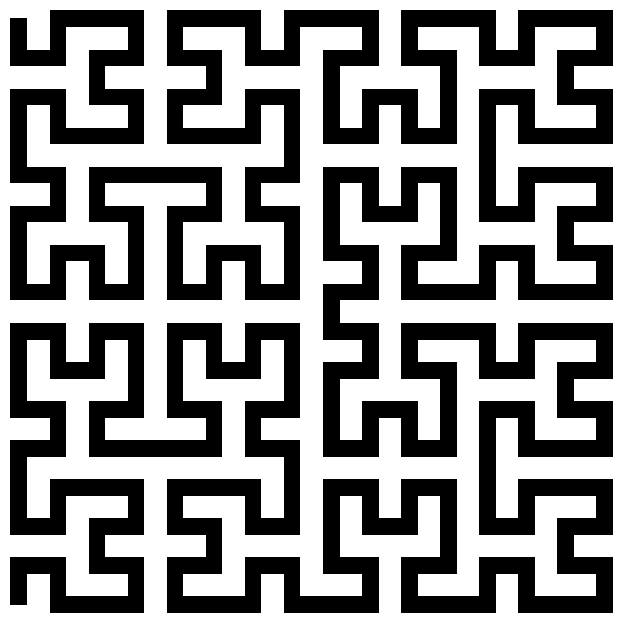
\includegraphics[height=2cm]{img/hilbert.ps}\\
Some Company\\
With it's address\\
ThePlace, the Netherlands\\
\httpurl{www.url.nl}
}

% Optional (postscript) cover picture. Put this in comments when not needed.
\coverpicture{\includegraphics[width=13cm]{img/maze.ps}}


% A copyright notice and maybe something about the cover picture
% Put in comments to get the default copyright notice
\colophon{\noindent
  \copyright{} 2014 \theauthor. \emph{Note that this notice is for demonstration
  purposes and that the \LaTeX{} style and document source are free to
  use as basis for your MSc thesis.} \\[1em]
  Cover picture: A ``random'' maze generated in postscript.
}

% thesis committee:
\chair{Prof.dr. A. Professsor, Faculty EEMCS, TU Delft}
\supervisor{Dr. S.T.A.F.F. Member, Faculty EEMCS, TU Delft}
% The following two are optional for LaTeX (current university
% regulations state that at least one of them should be assigned)
\externalsupervisor{Drs. E.X. Ternal, Some Company}
\committeemember{Dr. S.T.A.F.F. Member, Faculty EEMCS, TU Delft}


\setcounter{tocdepth}{1}
\setsecnumdepth{subsection}
\maxsecnumdepth{subsection}

\begin{document}

%---------------------------------------------------------------------%
%                     Custom commands                                 %
%---------------------------------------------------------------------%

\newcommand{\reff}[2]{\hyperref[#2]{{#1}\ref*{#2}}}
\newcommand{\refff}[3]{\hyperref[#2]{{#1}\ref*{#2}{#3}}}
\newcommand{\httpurl}[1]{\href{http://#1}{\nolinkurl{#1}}}
\newcommand{\mailurl}[1]{\href{mailto:#1}{\nolinkurl{#1}}}

%---------------------------------------------------------------------%
%                     Document start                                  %
%---------------------------------------------------------------------%

\frontmatter
\thispagestyle{empty}
\maketitle                                      % for the cover page
\makeformaltitlepages{\input{abstract}}         % for formal title pages with all info

\include{preface}

\cleardoublepage\tableofcontents
\cleardoublepage\listoffigures
\cleardoublepage\mainmatter

\include{introduction}
\chapter{Chapter Title}
\label{cha:title}

Short chapter intro \ldots

\section{A section}

A reference to \ref{cha:intro}.
Another reference to \reff{chapter~}{cha:intro}.
And again another reference to \refff{chapter~}{cha:intro}{a}

\lipsum{2} % add some pseudo content

\lipsum{2}

\section{Another section}

\lipsum{7} % add some pseudo content



\chapter{Related Work}
\label{cha:related}

(Your topic here) is a well explored domain in computer science. This
chapter discusses technologies related to (my research project). It is
divided into \ldots

\section{Related part I}

\lipsum{2} % add some pseudo content

\section{Related part II}

\lipsum{4} % add some pseudo content

\section{Related part III}

\lipsum{1} % add some pseudo content


\include{conclusions_and_future_work}

\cleardoublepage\backmatter

\bibliographystyle{plain}
\bibliography{thesis}

\appendix
\def\chaptername{Appendix}
\chapter{Glossary}
\label{cha:glossary}

In this appendix we give an overview of frequently used terms and
abbreviations.

\begin{description}
\item[foo:] \ldots
\item [bar:] \ldots
\end{description}


\include{requirements}

%---------------------------------------------------------------------%
%                     Document end                                    %
%---------------------------------------------------------------------%

\end{document}
